\documentclass[tikz,border=10pt]{standalone}
\usepackage{tikz}
\usepackage{pgfplots}
\pgfplotsset{compat=1.18}
\definecolor{local}{RGB}{75,171,224} % 4BABE0
\definecolor{remote}{RGB}{178,112,175} % B270AF
\definecolor{petals}{RGB}{210,127,72} % D27F48
\begin{document}
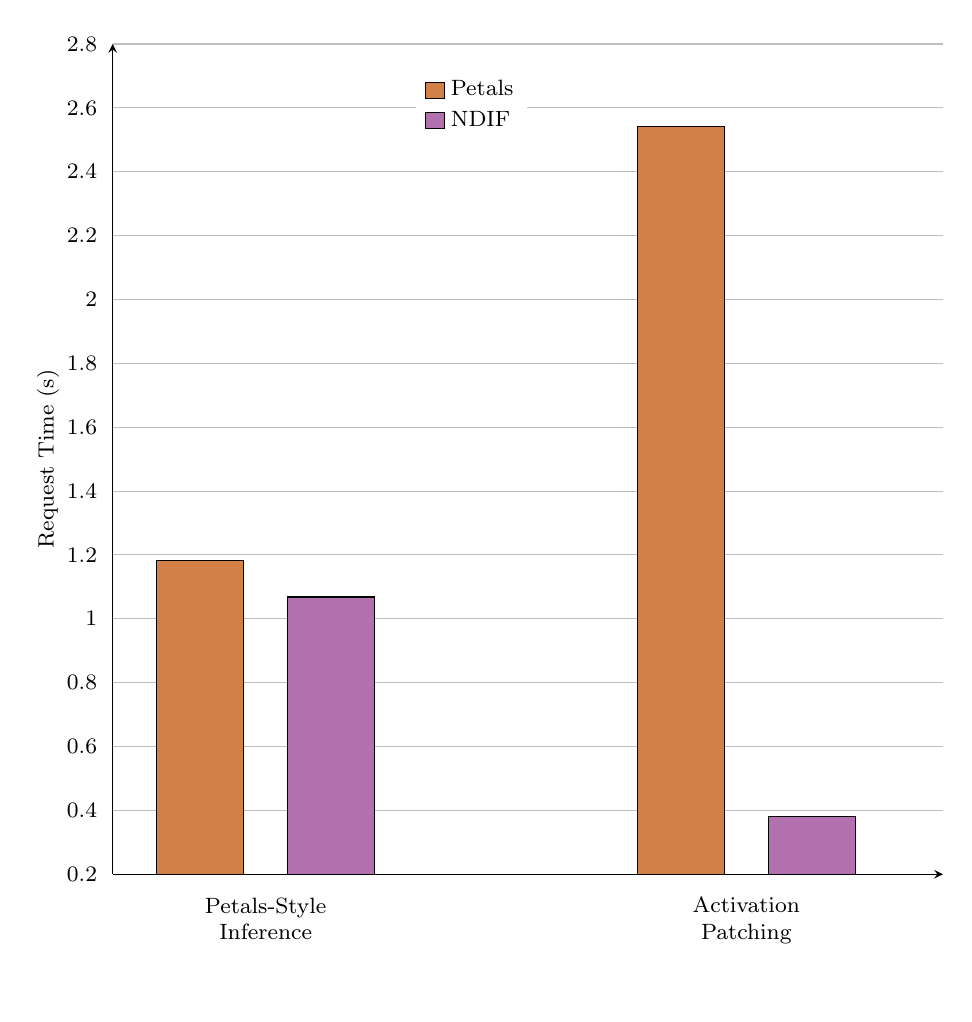
\begin{tikzpicture}
    \pgfplotsset{
        every x tick label/.append style={yshift=-0.3cm, font=\footnotesize},
        every y tick label/.append style={font=\footnotesize},
        xlabel style={font=\footnotesize},
        ylabel style={font=\footnotesize}
    }
    \begin{axis}[
        width=\textwidth,
        height=\textwidth,
        xtick={1.3, 3.5}, % Spacing between groups
        xticklabels={Petals-Style Inference, Activation Patching},
        ylabel={Request Time (s)},
        ylabel style={yshift=-4pt},
        xlabel={\textcolor{white}{Number of Parameters (log-scale)}},
        x tick label style={anchor=north, align=center, text width=1.8cm},
        xticklabel style={yshift=0.2cm}, 
        xmin=0.6,
        xmax=4.4,
        ymin=0.2,
        ymax=2.8,
        axis y line=left,
        axis x line=bottom,
        ymajorgrids=true,
        xtick style={opacity=0},
    ytick style={opacity=0},
        scatter/classes={
            a={petals}, % Group 1
            b={remote} % Group 2
        },
        legend cell align={left},
        legend style={
            draw=none,
            fill=white,
            font=\footnotesize,
            at={(0.5,0.97)}
        },
        legend entries={Petals, NDIF},
        legend image code/.code={
            \draw[bar width=0.4,fill=#1] (0cm,-0.1cm) rectangle (0.25cm,0.1cm);
        }
    ]

    %\draw[thick, dashed, color=local, line width=1.2] (axis cs:1,1.181540595224826) -- (axis cs:2,2.5427969290420522);

    \addplot[ybar, bar width=0.4, fill=petals] 
    coordinates {
        (1,1.181540595224826) [a]
    };
    %\addlegendentry{Petals}

    \addplot[ybar, bar width=0.4, mark options={scale=1.3}, fill=remote] 
    coordinates {
        (1.6,1.0681144390815558) [b]
    };
    %\addlegendentry{NDIF}

    %\draw[thick, dashed, color=remote, line width=1.2] (axis cs:1,1.0681144390815558) -- (axis cs:2,0.38146310793648225);

    \addplot[ybar, bar width=0.4, fill=petals] 
    coordinates {
        (3.2,2.5427969290420522) [a]
    };

    \addplot[ybar, bar width=0.4, mark options={scale=1.3}, fill=remote] 
    coordinates {
        (3.8,0.38146310793648225) [b]
    };

    \end{axis}
\end{tikzpicture}

% \begin{tikzpicture}[scale=0.7]
%     \begin{axis}[
%     %axis x line=center,
%     xtick pos=left,
%     ytick pos=left,
%     axis y line*=left,
%     axis x line*=left,
%     ylabel near ticks,
%     xlabel near ticks,
%     xlabel=Requirement (\#sentences),
%     ylabel=mean F1,
%     xtick={0, 1, 3, 4},
%     xtick
%     ]

%     \addplot[
%     scatter/classes={a={local}, b={remote}},
%     scatter,
%     only marks,%
%     scatter src=explicit symbolic,
%     nodes near coords*={\Label},
%     visualization depends on={value \thisrow{label} \as \Label},
%     ]%
%     plot [error bars/.cd, y dir = both, y explicit]
%     table[meta=class, x=x, y=y, y error=ey]{
%         x   y   ey  class   label
%         0   1.181540595224826  0   a   Petals
%         1   1.0681144390815558  0   b   NDIF
%         3   2.5427969290420522  0   a   Petals
%         4   0.38146310793648225  0   b   NDIF
%     };
%     \end{axis}
% \end{tikzpicture}
\end{document}